\chapter{音楽用語の定義}

本章では音楽用語の定義及びその説明を行う。

\section{音}

音とは、弾性体~(空気)~中を伝播する弾性波により起こされる音波が聴覚により感じられるもののことである。また、音波に周期性があり明確な音程を持つ音として聞こえる場合は楽音と呼ばれる。

\section{楽音の要素}

楽音は長さ,高さ,大きさ,音色の四つの要素から成り立ち~\cite{音楽の基礎}、人間はこれらを知覚することができる。本論文では楽音のことを音と呼ぶ。

\subsection{音の長さ}

音の長さは音波の時間の長さにより決まる。一般に、音の長さは楽譜上での時間の長さ~(音価)~により決まるが、本論文では音波の時間の長さにより決まるものとする。

\subsection{音の高さ}

音の高さは音波の周波数により決まる。人間には周波数が高い音は高く、周波数が低い音は低く知覚さる。また、複数の周波数の音波が音に含まれる場合は最も低い周波数成分の音波~(基音)~を音の高さとして知覚する。国際の音名表記では、C,D,E,F,G,A,Bを西洋音楽の七音音階におけるオクターブとして定め、それぞれのオクターブに番号を振り、440Hzの音をA4と定めることで、任意の半音の絶対的な表記を可能にしている。国際の音名表記では半音よりさらに細かい音~(微分音)~を表すことはできないが、本論文では扱わない。

\begin{figure}[t]
\begin{center}
\begin{minipage}{0.48\hsize}
\begin{center}
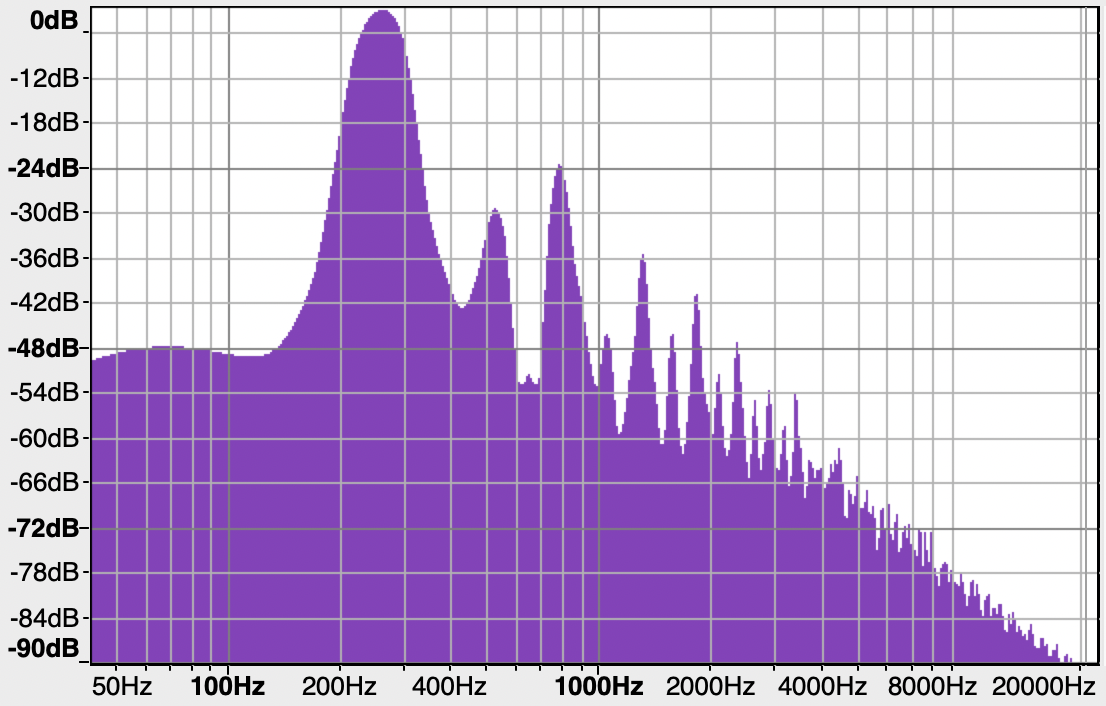
\includegraphics[width=0.95\hsize]{figure/c4_harp_spectrum.png}
\caption{音波の周波数スペクトル}
\label{fig:spectrum}
\end{center}
\end{minipage}
\begin{minipage}{0.48\hsize}
\begin{center}
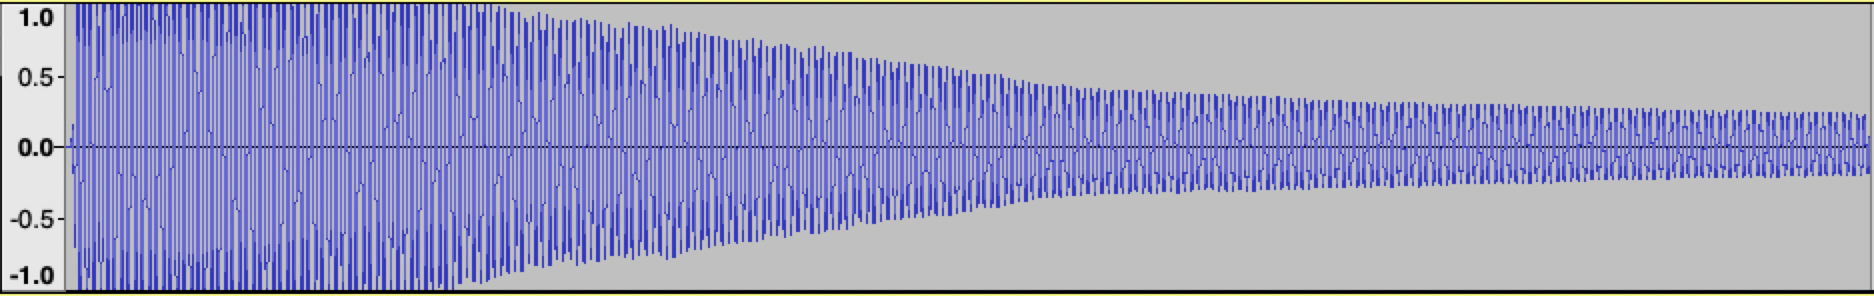
\includegraphics[width=0.95\hsize]{figure/c4_harp_wav.png}
\caption{C4の音波の波形}
\label{fig:wav}
\end{center}
\end{minipage}
\end{center}
\end{figure}

ここで、図\ref{fig:spectrum}は図\ref{fig:wav}で示されるある音波にフーリエ変換を行うことで得られる周波数スペクトルである。周波数スペクトルはそれぞれの周波数成分がどれだけその音波に含まれているかを示すので、この音波の基音は264Hzとわかる。

\subsection{音の大きさ}

音の大きさは音波の振幅により決まる。人間には振幅が大きい音は大きく、振幅が小さい音は小さく知覚される。

\begin{figure}[t]
\begin{center}
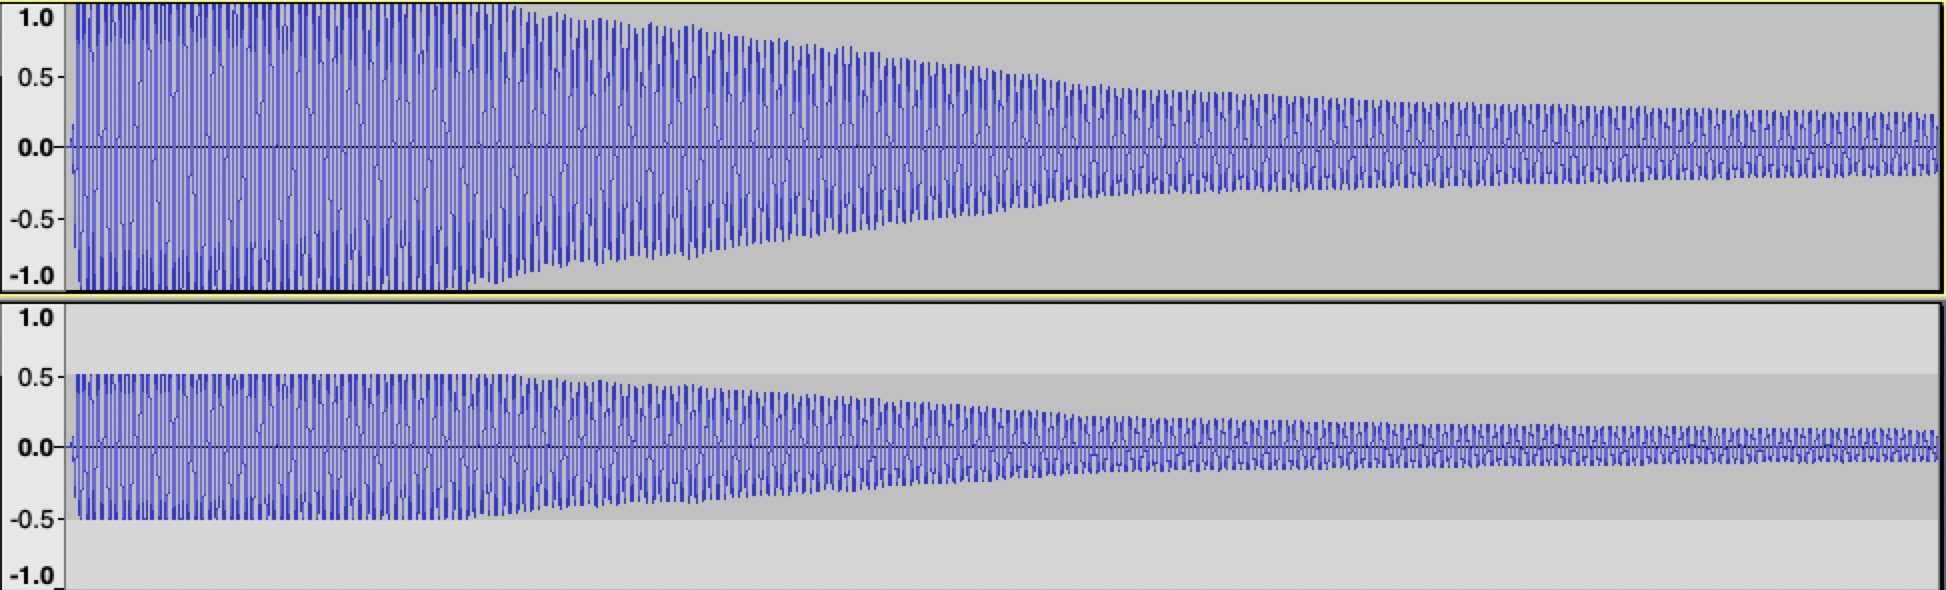
\includegraphics[width=0.7\hsize]{figure/c4_harp_loudness.png}
\caption{音の大きさの異なる音波}
\label{fig:loudness}
\end{center}
\end{figure}

図\ref{fig:loudness}では、同じ楽器から出る同じ高さの音の音波を示しており、振幅の大きい後者の方が大きい音として人間には知覚される。

\subsection{音の音色}

音の高さと大きさが同じであっても異なった音として人間には知覚されることがある。この違いを音色と呼ぶ。

\begin{figure}[t]
\begin{center}
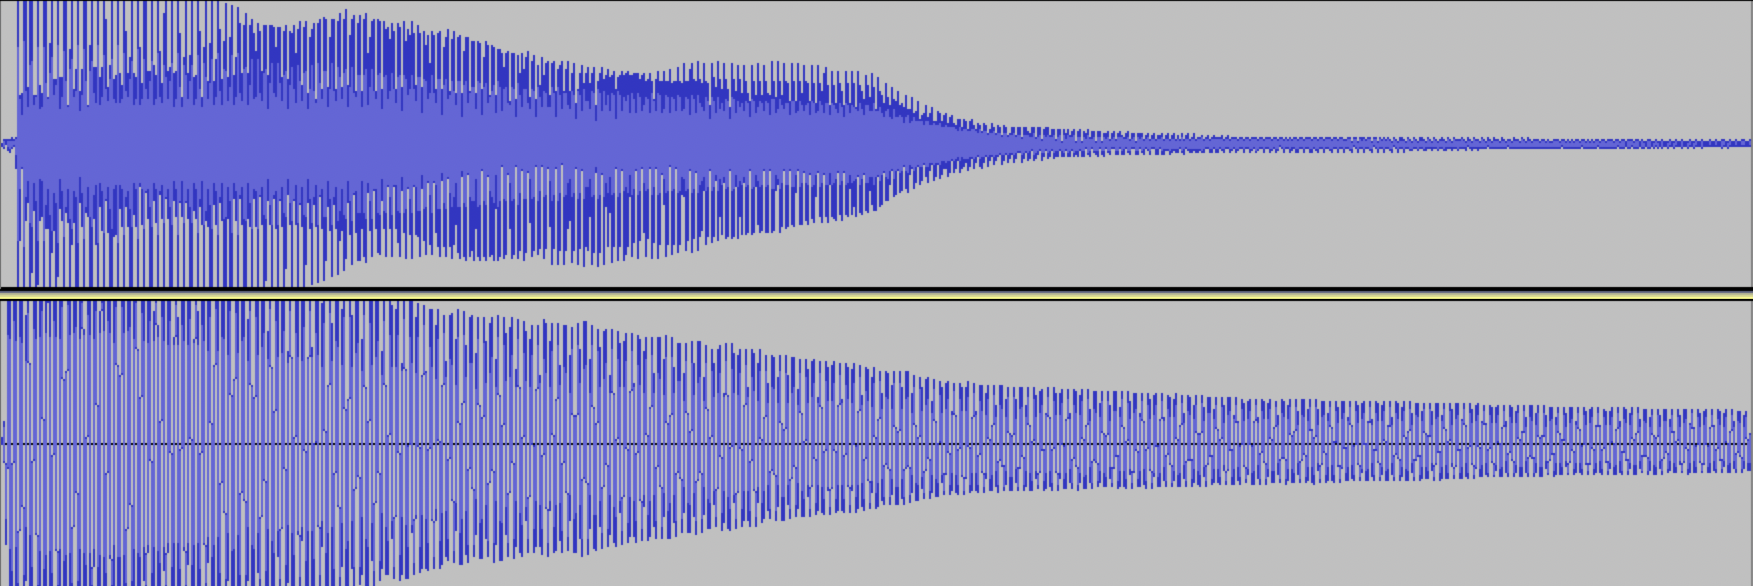
\includegraphics[width=0.7\hsize]{figure/c4_guitar_harp.png}
\caption{ギターとハープの音色}
\label{fig:guitar_harp_comp}
\end{center}
\end{figure}

図\ref{fig:guitar_harp_comp}では、上側はギターの音波,下側はハープの音波で同じ高さかつ同じ大きさであるが波形は異なる。音色の異なる音どうしは基音より高い音~(上音)~の組み合わせが異なるため、このような波形の違いが生まれる。この波形の違いが音色の違いを作り出す。
